\section{Time-of-Flight Market Research}

Since the semiconductors technology became fast enough for the development of ToF cameras in the year 2000, multiple companies developed image sensors for civil applications. The following section shall give an overview of the ToF cameras that are currently on the market or will soon be released. Detailed specifications like resolution, size, accuracy, hardware/software trigger and integration times can be found in the official associated datasheets. In the following table specifications of sample image sensors and complete camera systems from the industrial and consumer market are gathered:
\begin{center} 
	\begin{tabular}{| l | l | l | l | l | l | l |}
		\hline
		 & Pixel Array & Speed [fps] & FOV [$^\circ$] & Range [m] & Size [mm]  \\ \hline
		 Mesa SR4000 & 176x144 & 30 & $69x55$ & $8$ & $65x65x76$  \\ \hline
		 pmdtec CamBoardpico & 160x120 & 45 & $82x66$ & $1$ & $89x17x6$ \\ \hline		 
		 Fotonic E70 16W & 160x120 & 52 & $70x53$ & $30$ & $80x80x86$  \\ \hline
		 Argos 3D - P100 & 160x120 & 160 & $90x90$ & $3$ & $27x75x57$  \\ \hline
		 odos real.iZ-1K & 1280x1024 & 100  & not fixed & $10$ & $182x80x92$ \\ \hline
		 Basler ToF-6c & 640x480 & 30 & $48x38$ & $5$ & - \\ \hline
		 Microsoft Kinect 2 & 512x424 & 30 & $70x60$ & $8$ & $249x66x67$ \\ \hline
		 Polytec epc660 Sensor & 320x240  & 264 & - & $240$ & - \\
		 \hline	
	\end{tabular} \captionof{table}{Time-of-Flight camera systems}	
\end{center}
 The Argos 3D - P100 camera offers a high frame rate of 160 fps at a low depth resolution and number of pixels. It also has a hardware trigger which makes it useful for synchronization with other devices. Multiple sensors can be synchronized phase shifted to each other. The interaction of the IR light between different sensors is therefore prevented. The Real.iZ-1K brings the highest fps with the largest number of pixels. In contrast to the other system the pulsed wave ToF approach is used. Additional illuminators can be added to the camera to increase the accuracy at high distances. The standard C mount allows the exchange of the lens. Therefore, the field of view can be adjusted. The high flexibility of this system requires a calibration before it can be used. The output data must be preprocessed by a calibration matrix to obtain depth data. A trigger input allows the synchronization with other systems. The Fotonic E70 shows good motion blur characteristics and is the only sensor based on CCD technology. It is designed for rough environments and shows good outdoor characteristics. The company pmdtec offers ToF cameras, such as the highly compact Camboard Pico and the Camboard Nano, where the lenses and illuminators are fixed. Since there is no hardware trigger, a synchronization frame by frame is not possible. Mesa SR4000 is one of the pioneer in ToF technology. Lots of scientific work has been published based on this system. Basler is a new player is this sector, offering the first prototype with a high number of pixels at 30 fps and an external trigger. The Development of image senors with $1280x1024$ is already announced. Microsoft brings ToF with the Kinect 2 into the consumer market. Compared to the other industrial system, the price is very low with $200~\$$ for a complete development kit. Nevertheless the resolution, range and accuracy can still keep up. A higher frame rate and range has been implied \cite{payne20147} \cite{sell2014xbox}. A disadvantage is the absence of raw data access and low level configurations. Polytec makes a huge advantage with the image sensor epc660. 264 fps at 320x240 pixels should allow the investigation of fast dynamic scenes. A region of interest enables 4000 fps at 160x30 pixels and therefore various applications in the investigation of fast unsteady deformations. Currently there is no operational camera on the market with this sensor. Overall, the ToF market is rapidly growing. The cancelling of ambient light will allow outdoor applications soon, since companies like pmdtec are interested in outdoor application in the automotive industry. The increase in range, frame rate, depth resolution and number of pixels over the last few years enables many of industrial, civil and scientific applications. 

 \begin{figure}[!h]
 	\centering
 	\fbox{\includegraphics[width=0.37\linewidth]{Bilder/odos.jpg}}
 	\caption{odos real.iZ-1K 1280x1024 with changeable lens and illuminator}
 	\label{fig:odos_real_iK_1K}
 \end{figure} 


\subsection{Kinect 2 System Overview}
The Kinect 2 is the first Time-of-Flight consumer camera and brings the highest total amount of pixels compared to other ToF devices at the time of the release. It is originally designed for gesture recognition and enables the control of games and other applications by hand or body movements. This thesis concentrates on the ToF camera even if other sensors are included, like a microphone array and a HD CMOS rolling shutter camera for visible light. In contrast to the Kinect 1, the developer decided to change the technique of the range imaging from a structured light sensor to Time-of-Flight. This increases the accuracy, field of view, resolution, number of pixels and the maximum distance. Thus movements of multiple persons can now be captured in parallel and applications can be controlled by the users even by figure gestures. No official technical specifications of the sensor have been released yet. In Payne's publication, an image sensor is presented that probably is the one, which is integrated in the camera \cite{payne20147}. The following table represents the basic specifications from the publication:
\medskip

	\begin{center}
    \begin{tabular}{| l | l |}
    	\hline
    	Pixel Pitch & $10~u*10~u$  \\ \hline
    	Chip Size & $8.2~mm*14.2~mm$  \\ \hline
    	Pixel Array & $512 x 424$  \\ \hline
    	Dynamic Range & $>2500=68~db$  \\ \hline
    	Modulation Frequency & $10-130~MHz $ \\ \hline
    	Average Modulation Frequency & $80~MHz$ \\ \hline
    	Field of View &  70 (H) x 60 (V) degrees  \\ \hline
    	Depth Uncertainty & <0.5 $\%$ of range \\ \hline
    	Operating Wavelength & $860~nm$ \\ \hline
    	Frame Rate &  max. $60~fps$ (typical $30~fps$) \\ \hline
    	ADC Data Stream & $2~GS/s$ \\ \hline
    	Effective Fill Factor & $60\%$ \\ \hline
    	Reflectivity &	$15\%-95\%$ \\ \hline
    	Responsivity @ $860~nm$ & 0.144 A/W  \\ \hline 
    	Readout Noise	& $320~uV$ differential \\ \hline 
    	ADC Resolution & $10~Bits$ \\ 
    	\hline 
    \end{tabular} \captionof{table}{Kinect 2 system specifications}	
\end{center}
\newpage

The illumination is based on three $860~nm$ IR laser diodes. A rough measurement of the emitted light with a single IR photo diode and an oscilloscope showed that the diodes flash with a rate of $30~Hz$. The frame rate of the depth video stream also corresponds to $30~fps$, visible in figure \ref{fig:Kinect2_photodiode} and \ref{fig:Photodiode_measurement_kinect_3frequencies}. Every IR flash period comes with a burst of three different intensities and frequencies of $120~MHz$, $80~MHz$ and $16~MHz$ for a time of approximately $5.4~ms$ resulting in one depth frame \cite{sell2014xbox}. After about $16~ms$ of IR light, the diodes are turned off for $16~ms$ and a new image is created. The captures are taken in rapid temporal succession to avoid motion blur. Every image results out of three different modulation frequencies to achieve the high dynamic range over large distance from $0.5~m$ to $8~m$. Microsoft does not allow low level hardware access yet to change the modulation frequency or integration time.
The sensor diodes feature a responsivity of $0.14~ A/W$ at the laser wavelength. To increase the fill-factor to $60\%$, micro lenses are integrated into every pixel for a larger detecting area. With the given lens speed of 1.07, the focal length is approximately $80~mm$ with a aperture measured by hand of about $70~mm$. Figure \ref{fig:Kinect2_optic} shows a Kinect 2 disassembled. The three laser diodes are heavily shielded. The beam is scattered and filtered by the optic in front of the diodes. The IR camera lens and the case are equipped with monochromatic filters. Disturbing IR light sources such as the sun are reduced in this way.\\ 
 
 \begin{figure}[!h]
 	\centering
 		\fbox{\includegraphics[width=0.8\linewidth]{Bilder/IR_camera.jpg}}
 	\caption{Kinect 2 IR camera and IR illumination with scattering optic }
 	\label{fig:Kinect2_optic}
 \end{figure} 
 

A high dynamic range is necessary to simultaneously render high-reflectivity objects near the camera and low-reflectivity objects far from the camera to provide the depth resolution for all pixels. Every pixel selects the best shutter time and amplifier (AMPs) gain for the ADCs by itself. The digitized output from the ADCs is combined in the shutter engine. The MIPI interface provides the communication to other embedded systems. Figure \ref{fig:Kinect2_ImageSensor} shows a microscope image of the Kinect 2 Image Sensor. The electronic for the processing of the data is located on the sides to avoid interferences with the image sensor, common on modern CMOS sensors.\\

\begin{figure}[!h]
	\centering
	\includegraphics[width=0.5\textwidth]{Bilder/Kinect2Sensor.png}
	\caption{Kinect 2 image sensor \cite{payne20147}}
	\label{fig:Kinect2_ImageSensor}
\end{figure} 


A USB 3.0 connection allows the readout of the images with a latency less than $20~ms$. A $12~V$ power supply delivers additional power to the camera when it is plugged to a computer. The data and the power supply are combined in a proprietary cable. Thus, the Kinect Hub is required to use a standard USB 3.0 plug for the PC connection. With the Microsoft Software Kinect 2 Studio, the data steam can be observed in a 3D point cloud but direct access to raw data is not possible in this application. Microsoft offers the Kinect for Windows Development Kit 2.0 to create customized programs for the processing of the Kinect 2 data stream. Several demonstration programs with source code in $C++$ and $C\#$ are included but raw data acquisition of a complete video stream is not provided yet. Wai Ho Li offers the first open source tool dumpK4W that saves the "raw" data from the video stream to a mass storage \cite{dumpk4W}. These images are given in an integer resolution in millimeters and therefore the data stream must already be processed by the camera itself. Wai Ho Li uses the OpenCV library for real-time computer vision to save every picture from the data stream. The images cannot be processed in real-time for further investigations. A driver for the Matlab environment would be useful for a real-time processing.\\

The field of view of the IR camera is fixed to one lens position. Adjustment of the focal length is not possible. The advantage for the user is, that the system can be calibrated before it is shipped to the customer. A calibration before the operation of the camera is therefore not necessary. The range images are converted into millimeters inside the camera before they are transfered via USB. The area $A$ that is observed by the sensor in a certain plain results out of the distance and the angle of view $\theta$ in the horizontal and vertical direction: 

\begin{equation}\label{eq:lfov}
l_{h,v} = \tan{\frac{\theta_{h,v}}{2}}\cdot d \cdot 2~[m]
\end{equation}

\begin{equation}\label{eq:area}
A = l_v\cdot l_h = \tan{\frac{70^\circ}{2}}\cdot \tan{\frac{60^\circ}{2}} \cdot d^2 \cdot 4~[m]
\end{equation}
\medskip
The area projected on a single quadratic pixel $A_i$ is the fraction of one pixel to the complete area $A$. Figure \ref{fig:FOV} illustrates the field of view, the distance to the observed scene d, the coordinate system of the observed plane (index p) and the camera (index c).

\begin{equation}
A_i = \frac{A}{512\cdot 424}~[m^2]
\label{eq:pixel_area}
\end{equation}

\begin{figure}[!h]
	\centering
	\includegraphics[width=0.53\textwidth]{Bilder/425px-Angle_of_view.pdf}
	\caption{Kinect 2 field of view}
	\label{fig:FOV}
\end{figure} 


\section{Data Processing of Range Images}
The video stream, saved with dumpK4W, consists of a bunch of individual pictures. A frame rate of $30~fps$ every second of acquisition will result in 60 images from the IR camera. One capture is represented in a depth and intensity image. The data is given in the Tagged Image File Format (TIFF) in 512x424 pixel with a non-standard aspect radio. TIFF is a common format for the lossless storage of image data. The pixels consist of a $16~Bit$ integer number that represents the distance in millimeters to the image plane. About 13 bits are used corresponding to the $8000~mm$ of maximum distance. Values under $500~{mm}$ and beyond $8000~{mm}$ are set to zero. 
 When opened in a standard image viewer, the files seem to be only black. The brightness and the contrast must be changed to foreground the shades of grey to distinguish different pixels. Matlab provides a set of tools for the processing of the raw data. The Matlab Image Processing Toolbox delivers a variety of ways for the processing of images and video streams. It is widely used in scientific environment and features offline and live processing of image data. Figure \ref{fig:imagesc} represents a raw image that is plotted with the imagesc() function in Matlab.  

\begin{figure}[!h] 
	\centering
	\includegraphics[width=1.0\textwidth]{Bilder/2m_bass_office.png}
	\caption{Raw image plotted with imagesc() function}
	\label{fig:imagesc}
\end{figure}   

The distance is represented in a red, green and blue colorspace that is fitted to the depth resolution. Red indicates far distances and blue the near fields. Isolines in the color space show equal regions of distance. Figure \ref{fig:imagesc} shows, that the depth values are given perpendicular to the image plane. The isolines run parallel to the image plane, possible due to the fixed calibrated focal length and simplifies the processing of the data considerably.
Noise is one of the major challenges in the interpretation of ToF Data. It can be considered as an unwanted fluctuation of the range measurement error. The noise increases at the corners of the FOV. This is caused by the optic of the camera and the light cone of the illumination. The lens reduces the light intensity at the outer boarders of the image. The threshold in this area can barely be archived and therefore the Signal-to-Noise ratio is reduced. The live display of the point cloud in Kinect Studio can be used for a rough estimation of the noise. The pixels seem to jump when observed live on a static surface. A detailed analysis of the noise characteristics can be found in section \ref{sec:static_evaluation}. The orientation of the raw data is flipped in the vertical axis, since it is given in the camera coordinate system. The Matlab command fliplr() transforms the image into the observed plane coordinate system.

\subsection{Transformation into Point Cloud Data}
The data must be transformed into a so called point cloud to gain 3D information out of the 2D data. The images are already given in a calibrated form happens inside the camera. Other camera devices with adjustable FOV, low level configuration and flexible illumination need a calibration of the raw images into the corresponding distance. Systematic errors are reduced in this way \cite{lindner2010time} \cite{lefloch2013technical}. Every pixel in the $512x424$ array corresponds to a single point in 3D space, depending on the field of view and distance. Kinect Studio enables to rotating of live point cloud data. The regions which are not reached by the IR light, are highlighted in the form of shadows. Figure \ref{fig:pointcloud} shows one frame of the video stream that is shifted to the perspective of the camera. The person in the foreground shows an ideal diffuse reflection of the IR light and therefore a high signal-to-noise ratio. The transformation into a point cloud from raw data is also possible with the open source program MATLAB to Point Cloud Library (PCL) created by Peter Corke. It delivers a bundle of tools for visualization, surface reconstruction, filtering and segmentation. It is a standard environment for 3D image processing, that is developed by companies from different industries.

\begin{figure}[!h]
	\centering
	\fbox{\includegraphics[width=0.9\textwidth]{Bilder/pointcloud.png}}
	\caption{Point cloud in kinect studio}
	\label{fig:pointcloud}
\end{figure}  


\newpage
\subsection{Meshing of Point Cloud Data}
For the reconstitution of a scanned object, 3D points are not enough. The point cloud needs to be meshed. The vertices in the form of points represent knots for this connection. The lines in between are called edges. A face is a set of edges that can be combined into a closed surface. Figure \ref{fig:Mesh_overview} shows the transformation of a cube from vertices to triangle faces. 

\begin{figure}[!h]
	\centering
	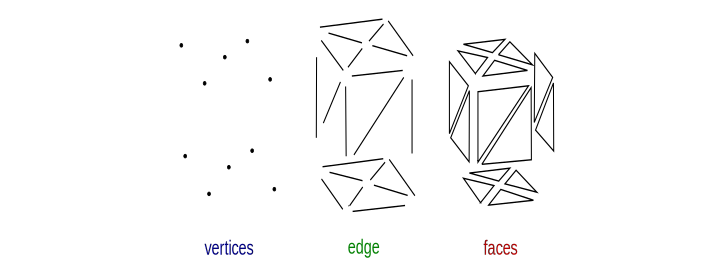
\includegraphics[width=0.8\textwidth]{Bilder/Mesh_overview.pdf}
	\caption{Transformation from vertices into faces \tiny Rchoetzlein wikipedia.org \ccbysa}
	\label{fig:Mesh_overview}
\end{figure}

Kinect Fusion is a Simultaneous Localization and Mapping (SLAM) algorithm which is capable to mesh the ToF video stream in real time. It is designed for accurate real-time mapping of complex and arbitrary indoor scenes. The algorithm is capable to recalculate the camera's orientation and position when it is moved. In the Kinect Fusion Explorer Demo, Microsoft allows the export of this data into a mesh format like the Surface Tesselation Language (STL). It is a standard interface that is supported by most 3D programs for further processing. 
Stlwite is another tool for Matlab to create STL files from the raw depth data. Figure \ref{fig:AC_meshing_Meshlab} shows a single frame of an aircraft model that is taken with the Kinect 2 camera, transformed into STL with Matlab and imported into the Open Source program Meshlab. Data from the far background and foreground was removed from the point cloud in Meshlab. The flying pixels at the edges lead to "flying surfaces" after the meshing of the raw image. 

\begin{figure}[!h]
	\subfigure[Meshlab]{\includegraphics[width=0.4\textwidth]{Bilder/meshedaircraft.png}\label{fig:AC_meshing_Meshlab}}\hfill
	\subfigure[Matlab]{\includegraphics[width=0.6\textwidth]{Bilder/ACMesh.png}\label{fig:AC_meshing_Matlab}}
	\caption{Meshing of point cloud data}
\end{figure}

The camera must be moved to provide a complete 3D scan of an object from all sides. To fuse multiple images into a single 3D space, the orientation of the object to the camera must be know. Reconstruct Me and other software toolkits offer the scan of a room or objects from different points of view. The position of the moving camera is calculated out of the video stream. By merging the range data from all sides, the 3D scape is reconstructed. 

A simple construction of mesh data from range images can also be done in Matlab. The function mesh(Z) draws a wireframe with a surface color corresponding to the Z axis. It is a simple and fast way to determine the quality of the raw data. Before the meshing of the image, it needs to be transformed in double values by the function double(). For a reduction in processing time, the data can be reduced to the distance of the investigated object. Measurements in other regions are cut out. The data cursor in an already plotted mesh helps to identify this value by the user. Figure \ref{fig:AC_meshing_Matlab} shows the resulting plot and the cursor to identify the region of interests with a cut off distance of 800 mm.
\medskip
\begin{lstlisting}
Imagedouble = double(ImageInteger)
Imagedouble(Imagedouble > CutoffDistance) = 0
mesh(Imagedouble)
\end{lstlisting}

\
\subsection{Analysis and Filter Methodes} 
 Multiple filtering approaches are made, to improve the quality of the image data. They all have in common that they aim to remove the measurement noise which results from different types of error specified in section \ref{chap:range_errors}. Fluctuations between multiple depth images are useful to separate noise from the so called ground truth image. 

\subsubsection{Creation of Frame Arrays} \label{chap:Framearray}
For the processing of a video stream the single pictures have to be aligned into a single matrix that consists out of the rows times columns times number of images L. 90 frames for example recorded in $3~s$ create an 512x428x90 3D matrix called Framearray. The data is gathered from a folder that contains all depth images. For keeping them in the right order, they have to be numbered consecutively in the file name. The time delta between two frames correspond to $T_{sampling} =\frac{1}{fps}$. The following code shows how to create an array of frames in Matlab out of an image folder. The images are transfered into double data type from unsigned integer.
\medskip
\begin{lstlisting} 
ImageFolder=uigetdir('C:\ImageFolder','Folder RAW Data Images');
L=length(dir(strcat(ImageFolder,'\*.tiff')));
for g = 1:L
	Frame=double(imread(strcat(ImageFolder,'\',tiffFilesS(g).name)));;
	Framearray(:,:,g) = Frame;
end
\end{lstlisting} 

\subsubsection{Mean and Variance}
The ground truth image is simply the mean of all data from the stream. Noise in the depth information is canceled out by multiple measurements. This is a standard way to remove non-systematic noise for a higher precision. The additional parameter in the function declares the dimension over which the matrix is averaged. The number of images determines the quality of the result. In some publications up to 500 images are used. Movements in the recording time corrupt the resulting image.
\medskip
\begin{lstlisting}
GroundTruthImage = mean(Framearray,3) 
\end{lstlisting} 
\medskip
The variance of a single pixel depth measurement versus time determines how much the value fluctuates around the mean value. With the ground truth image as the expected value $\mu$ the variance \ref{eq:var} of a single pixel can be derived with the Var() function:
\medskip
\begin{lstlisting}
PixelVariance = var(Framearray(Colume,Row,:));
\end{lstlisting}

\begin{equation}\label{eq:var}
\sigma^2(X)=Var(X)=\sum_{n=1}^N (x_i -\mu)
\end{equation}

The variance for an complete depth image plotted into a new image provides a simple way to estimate noise characteristics of different material. Figure \ref{fig:variance_raw} represents the variance of a scan on wooden plane area in a distance of about $700~mm$. Values with a higher variance than 7 mm are set to zero. The reason for that is the high amount of noise in the corners of the image. The variance reaches values up to $470~mm$, corresponding to the low radiant flux and darkening of the lens in the corners. The distribution is separated in elliptic uniform regions. The middle of the field of view shows the lowest variance. The variance increases in the image's corner direction. Apart from the corners, the variance alternates between 2 mm to 0.8 mm. In a box between 100 to 450 pixel horizontal and 50 to 350 pixel vertical the mean variance is 1.205 mm. Source code \ref{list:FFT} demonstrates the principle how the variance image can be created. The mean variance in a pixel area delivers a single value that is better comparable.

\begin{figure}[!h]
	\centering
	\includegraphics[width=0.85\textwidth]{Bilder/variance_platte_07m.png}
	\caption{Raw variance of an wooden plate in $700~mm$ distance}
	\label{fig:variance_raw}
\end{figure}

\newpage

\subsubsection{Gradient}
The gradient of an image specifies the alteration in the 2D data space. Mathematically the gradient of a two-variable function at each image pixel is a 2D vector with the components given by the derivatives in the horizontal and vertical direction. At each image point the gradient vector points in the direction of the largest possible intensity increase. The length of the vector is a measure for the rate of change. The gradient of an image is given by the formula with x pointing in the horizontal and y in the vertical direction:

\begin{equation}\label{eq:grad}
\nabla f = \frac{\delta f}{\delta x} \hat{x} + \frac{\delta f}{\delta y} \hat{y}
\end{equation}
\medskip
\begin{lstlisting}
[Gmag,Gdir] = imgradient (Frame)
\end{lstlisting}
\medskip

The corresponding Matlab function imgradient() contains the magnitude of the vector Gmag and  the direction Gdir in degree to the vertical axis. The following Figure \ref{fig:gradient_magnitude} shows the image gradient of the office room. Values above $200~mm$ have been cut off to fit the colorspace and to highlight small differences.

\begin{figure}[!h]
	\centering
	\includegraphics[width=1\textwidth]{Bilder/OfficeGradientMag.png}
	\caption{Gradient magnitude of the office room}
	\label{fig:gradient_magnitude}
\end{figure}

The cupboard in front of the image stands parallel to the image plane. That is why the gradient is small. The floor features small changes in the foreground and with higher distance the magnitude increases. At the end of the room with a distance of $6812~mm$ the noise increases the gradient. Ideally, the flat wall should show only one constant value like the cupboard in the foreground. In general, high angles to the image plane will result in high gradients and low angles in small ones. This can be useful in different subjects. Edges around surfaces and planes are recognized. Flying pixels can be removed from the image, since they feature a high gradient to nearby pixels. Plane regions with various gradients conclude to areas with low reflectance or saturation of the image. The flat area in the middle shows a very low gradient and is therefore perpendicular to the sensor plane. 

\subsubsection{Denosing with Mean or Median of a Pixel Area}
One basic approach to reduce the noise in the depth data is the mean or median between nearby pixels. The depth is smeared to a single value. Such kind of filtering benefits from the Kinect's high number of pixels. The median sorts every element by its value and takes the middle element. Therefore, the impact of outlier can be reduced. The mean sums up every value and divides it by the number of elements. The following source code shows the calculation of a median and a mean value from a pixel area:

\begin{lstlisting} 
for g = 1:NumberOfPictures
    k=0;
    for a=1:v_windowlength 
   		for b=1:h_windowlength
   		k=k+1;
   		Pixelsector(k) = FramearrayDyn_Raw(v_edge+a,h_edge+b,g);                
    		end
    end
    DynPixelMean(g) = mean(Pixelarea); 
    DynPixelMedian(g) = median(Pixelarea);
 end
\end{lstlisting}

A pixel area with the vertical dimension v$\_$windowlength and horizontal dimension h$\_$windowlength is collected in the array Pixelsector. The postion is determined by v$\_$edge and h$\_$edge. DynPixelMedian collects the median value of this area for every pixel.
   
\subsubsection{Total Variation Denoising}

Rudin et al. pioneered the Total Variation Denosing (TVD) filter method that suppress noise profiles like Gaussian noise. In contrast to other approaches, like linear smoothing or median filtering, TVD simultaneously preserves edges whilst smoothing away noise in flat regions, even at low signal-to-noise ratios. It is based on the principle that signals with excessive and possibly disturbing details have high absolute gradients \cite{rudin1992nonlinear}. With a given signal, the absolute gradient can be calculated by the following formula:

\begin{equation}
V(X)=\sum_{n} |(x_{i+1} - y_n)|
\end{equation}

One measure of closeness is the sum of square errors:

\begin{equation}
E(x,y)=\frac{1}{2}\sum_{n} (x_n - y_n)^2
\end{equation}

The aim of TVD is to minimize the following discrete functional versus the function $y_n$:
\begin{equation}
E(x,y_n)  + \lambda V(y_n)
\end{equation}

The regularization parameter $\lambda_r$ controls the impact of the total variation on the smoothing. A high value will minimize the total variation while small values will preserve the original signal. Figure \ref{fig:TVD_1D} plots a noisy signal and the filtered curve after TVD.

\begin{figure}[!h]
	\centering
	\includegraphics[width=0.5\textwidth]{Bilder/TVD_1D_Example.png}
	\caption{Total Variation Denoising of a 1D signal \tiny MAL 2010 wikipedia.org \ccbysa}
	\label{fig:TVD_1D}
\end{figure}

Noise from 2D data like range images helps significantly in the reduction of different noise qualities. An adaptive TVD approch is proposed based on an extended structure tensor using the amplitude and phase of the ToF signal as reference \cite{lenzen2011denoising}. In contrast to other filter methods, depth noise is removed from the 3D shape, while edges are still preserved. This algorithm has been implemented by Guy Gilboa into Matlab \cite{TVD_Matlab_code}. $\lambda$ is set to one by default. The number of iterations is adjustable. Even if we cannot access the phase and amplitude of ToF data, the filter can still be used on the raw images with fixed parameters. Figure \ref{fig:variance_TVD} illustrates the variance of the same data which figure \ref{fig:variance_raw} is based on. The TVD filter significantly reduced the mean variance of the complete plate from $1.205~mm$ to $0.1540~mm$ based on 20 iterations and $\lambda_r =1$. The circular isolines of variance are highly reduced. Except for the corners, the variance could be reduced.

\begin{figure}[!h]
	\centering
	\includegraphics[width=0.9\textwidth]{Bilder/variance_platte_07mTVD.png}
	\caption{TVD filtered variance of an wooden plate in $700~mm$ distance}
	\label{fig:variance_TVD}
\end{figure}

\newpage
\subsubsection{Processing of Dynamic Depth Data} \label{sec:Dynamic_pixel}
The range information that is represented in the whole picture allows an dynamic investigation on every region of the field of view. For this purpose, the amplitudes of the noise must be smaller than the dynamic that is investigated. The number of images should correspond to $2^n$ for the FFT algorithm. If this is not the case, the remaining data is set to zero, fitting to $2^n$ samples. A new 2D array with the depth of every frame is created to investigate a single pixel over the complete video stream. Afterwards, the static offset of the data to the image sensor plane is removed. Every value of the array is reduced by the mean of the whole data set. Following this, the dynamic is investigated without the static offset to the surface. This process can be done for every pixel in the field of view. It remains a video stream, which contains just the dynamic. Out of this, new images are generated that represent the amplitude or frequency of the maximum peak in the spectrum. Source code \ref{list:FFT} shows how to create frequency and amplitude images out of the FFT. The variable $f_{p}$ represents the frequencies between zero and the maximum possible value of $15~Hz$. AmpsDyn contains the amplitudes $A_{p}$ divided by four and is given in the same dimension as the frequency array. The abs() function removes the complex values which result from the FFT and only the real part remains. The max() function returns the maximum values from the spectrum that we need to create the images for the $f_{p}$ frequency and $A_{p}$ amplitude distribution. Figure \ref{fig:Leinwand_FFT} illustrates the maximum amplitudes of a canvas in a frame that is excited with about $5~Hz$ by a student over 8 seconds. Higher values than $40~mm$ have been cut out to distinguish small changes in the color space.

\begin{figure}[!h]
	\centering
	\includegraphics[width=0.9\textwidth]{Bilder/leinwand.png}
	\caption{Peak amplitudes of every pixel of a canvas excited by a person}
	\label{fig:Leinwand_FFT}
\end{figure}

For a better investigation of the image, a cursor can be used to investigate the dynamic of a single pixel or a pixel area. Figure \ref{fig:timedomain_leinwand} shows the time domain and figure \ref{fig:frequencydomain_leinwand} the frequency domain of a pixel in the region of the excitation. The highest peak indicates the dominating frequency $f_p\approx 4.8~Hz$ in the spectrum at an dominating amplitude $A_p\approx 15~mm$. The second peak at about $2.5~Hz$ results out of the offset of the signal. The first harmonic emerges at about $9.6~Hz$. Every periodic signal consists of the dominating frequency $f_p$ and its harmonics, which are integral multiples of the dominating frequency $f_p$. The strongest harmonic peak is indicated as $f_{ph}$ and $A_{ph}$.


\begin{figure}[!h]
	\centering
	\includegraphics[width=0.8\textwidth]{Bilder/leinwandtimedomain.png}
	\caption{Time domain of excitation area}
	\label{fig:timedomain_leinwand}
\end{figure}

\begin{figure}[!h]
	\centering
	\includegraphics[width=0.8\textwidth]{Bilder/leinwandfrequencydomain.png}
	\caption{Frequency domain of excitation area}
	\label{fig:frequencydomain_leinwand}
\end{figure}

\newpage

\section{Data Processing of Laser Doppler Vibrometer} \label{chap:LDV_processing}
As an accurate and precise contactless measurement reference for the ToF camera, a Laser Doppler Vibrometer (LDV) runs parallel to the Kinect 2. The signal is transformed from fiber optic into a voltage signal, it is filtered and amplified before it is measured inside the Agilent DSO6054A oscilloscope. A digital interface delivers the access to the scope data. High sampling rates of common devices require a fast connection to gather the raw data over a long time. The digital resolution and sampling rate can also be reduced before it is transferred. Therefore, the data can be stored on a common USB stick in time domain CSV format. Columns are separated by comas and raws by new lines. This returns the time versus the voltage of every data point in two arrays of the same dimensions; Volt and Second. Equation \ref{eq:scope_capture} presents the way, how the reduced sampling rate is calculated depending on the TimePerDIV configuration on the screen, the number of samples $n_{samples}$ that are taken and the 10 rasters on the screen. TimePerDIV is adjusted by the knobs on the scope screen and $n_{samples}$ in the configurations.

\begin{equation}
\label{eq:scope_capture}
f_{sample}= \frac{n_{samples}-1}{TimePerDIV\cdot 10}
\end{equation}
\medskip

The time between every datapoint is the periode $T_{sample}$ and is used for the scaling of the time axis in the time domain and for the FFT analysis. 

\begin{equation}
\label{eq:sampling_period}
T_{sample}= \frac{1}{f_{sample}}
\end{equation}

For the transformation of the alternate voltage $U(t)$ in a corresponding speed $v$, the sensitivity $E$ adjusted at the LDV at the time of the measurement needs to be known. The CSV file format of the raw data can simply be imported in Matlab and transformed by equation \ref{eq:speed_transformation}.

\begin{equation}
\label{eq:speed_transformation}
v(t) = U(t) \cdot E
\end{equation}

 The direct current noise voltage needs to be removed from the data. This is done by a reduction of every value by the mean of all data. A better way would be to use a real high pass filer to remove the DC parts. The data needs to be integrated to get the displacement $z_{dyn(t)}$ from the speed v(t). The library offers a function cumtrapz() for this purpose. It computes an approximation of the cumulative integral via the trapezoidal method. The following source code extract shows the processing of the LDV data:

\begin{lstlisting} 
% Scope and Laser Doppler Vibrometer Data
E = 125 %%(mm/s)/V
n_samples = 1001; % zero based
TimePerDIV= 0.5 %s
f_samples = (n_samples-1)/(TimePerDIV*10);
speed =(Volt-mean(Volt))*E;
displacement=cumtrapz(speed)/f_samples; 
second=second+max(second);
\end{lstlisting} 

In the last step the time vector is corrected to start at zero. Afterwards, the displacement array can be processed in the same way as described in section Dynamic Analysis of Pixels \ref{sec:Dynamic_pixel}. The integration acts like a low pass filter. Sharp edges are removed and a smooth sinus remains. Equation \ref{eq:speed_sinus} shows the analytic mathematical integration of the speed to obtain the displacement. The constant offset $c$ must be calculated from other boundary conditions. This is helpful for a rough estimation of the displacement $z(t)$, directly at the scope with just the frequency $f$, sensitivity $E$ and the speed $v(t)$. The complete source code of the LDV data processing, which is done later in the experimental setup, can be found in the source code extract \ref{list:LDV_FFT}.

\begin{equation}
\label{eq:speed_sinus}
z(t)=\int v(t) dt = \int Asin(2\pi f t ) dt = -\frac{A}{2\pi f} cos(2\pi f t)  + c
\end{equation}


\begin{figure}[!h]
	\centering
	\includegraphics[width=0.7\textwidth]{Bilder/LDV_Row_data.png}
	\caption{$3~Hz$ Oscillating row data sampled with a scope}
	\label{fig:LDV_raw_Data}
\end{figure}

\newpage